\chapter{Timbre Similarity}  \label{musly}

\section{Gaussian Mixture Models of MFCCs}

\section{Construction Noise}
Comparing a construction noise sound sample with the private music collection containing mostly metal, rock, pop, classical and hip hop music, the following six best results could be achieved in descending order: 

\begin{itemize}
	\setlength\itemsep{0em}
	\item Ziegenm\"uhlen Session - Down On The Corner (Folk Musik)
	\item While She Sleeps - The Divide (Metalcore)
	\item Delain - Mother Machine (Live) (Symphonic Metal)
	\item Within Temptation - Sanctuary (Intro Live) (Symphonic Metal)
	\item Without A Martyr - Medusa's Gaze (Death Metal)
	\item 100 Meisterwerke der Klassik - Orpheus In The Underworld (Orph\'ee aux enfers) - Can-Can (Live At Grosser Saal, Musikverein) (Klassik)
\end{itemize}
Figure \ref{const1} and \ref{const2} show the distribution of the genres of 100 most similar songs compared to the construction noise sample.  

\begin{figure}[htbp]
	\centering
	\framebox{\parbox{1\textwidth}{ 
			\begin{subfigure}{0.49\textwidth}
				\centering      
				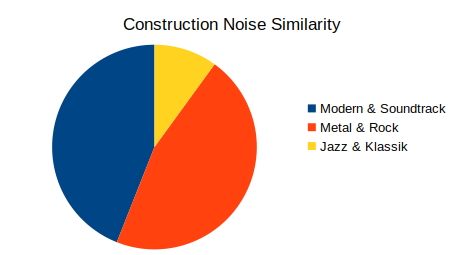
\includegraphics[scale=0.45]{Images/cnoise1.png}
				\caption{Similar genres to construction noise sample file}
				\label{const1}
			\end{subfigure}%
			\begin{subfigure}{0.49\textwidth}
				\centering 
				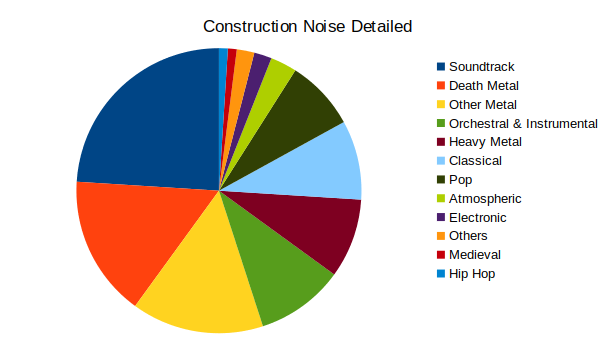
\includegraphics[scale=0.45]{Images/cnoise2.png}
				\caption{Similar genres to construction noise sample file in detail}
				\label{const2}
			\end{subfigure}
	}}
	\caption{Construction Noise}
	\label{fig:constn}
\end{figure}

Using the full dataset consisting of the private music collection, private field recordings, the full fma-dataset and the musicnet data, the following results could be achieved: 

\begin{itemize}
	\setlength\itemsep{0em}
	\item Born Pilot - Birds Fell (FMA, Electronic, Noise)
	\item mrandmrsBrian - sun is boring (FMA, Avant-Garde, field recordings)
	\item steps in snow (private field recording)
	\item Sawako - Paris Children (FMA, field recordings)
	\item Jeremy Gluck and Michael Dent - Olivier (FMA, Ambient Electronic)
	
\end{itemize}

\section{Different recordings and cover versions}
Another experiment was, to get the most similar songs to the famous 'Rondo alla Turca' by Mozart.
The recording used as a starting point is from the CD "100 Meisterwerke der Klassik" and has a length of 3:33 minutes.
This piece by Mozart appears overall four times in the dataset and is recorded by different pianists.
Every recording has a different length as listed in the following overview of the recordings by CD

\begin{itemize}
	\setlength\itemsep{0em}
	\item 100 Meisterwerke der Klassik (3:33)
	\item Piano Perlen (3:30)
	\item The Piano Collection - Disk 18 (3:28)
	\item Mozart Premium Edition - Disk 31 (4:29)
	
\end{itemize}
The top ten most similar songs to the 3 minutes and 33 seconds version are listed below:
\begin{itemize}
	\setlength\itemsep{0em}
	\item Mozart - Concert No. 10 for 2 Pianos and Orchestra in E Flat Major, KV 365 - 2. Andante
	\item Schubert - Sonata in B Flat, D. 960 - III. Scherzo (Allegro vivace con delicatezza)
	\item Albeniz - Iberia, Book I - Evocaci\'on
	\item Mozart Sonate Nr. 11 in A-Dur, K. 33 - Mozart - Alla Turca Allegretto (3:28)
	\item Beethoven - Bagatellen Op 119 -Allemande in D major
	\item Mozart - Rondo No. 1 in D Major, K. 485
	\item Mozart - Sonata For Piano No. 8 KV 310 A Minor - Allegro Maestoso
	\item Sonata For Piano No. 16 KV 545 C Major - Rondo: Allegretto
	\item Mozart Sonate Nr. 11 in A-Dur, K. 33 - III. Tuerkischer Marsch (3:30)
	\item Mozart - Piano Sonata No. 13 in B flat major, K. 333 (K. 315c): Allegretto grazioso
	
\end{itemize}

The interesting conclusion is that only 2 out of the 3 other versions were considered as most similar songs.
The slower recording wasn't even in the top 30 list of the most similar songs. 
The same was observable for other cover versions of songs in the dataset like Serj Tankians song "Lie Lie Lie" from the CD "Harakiri" and an orchestral recording of the same piece. 
This is probably due to the usage of GMMs of MFCCs representing and valuing the timbre of the music predominantly instead of the pitches.

\section{Conclusions}

Why using a big data framework would help: 
music similarity is not well defined. It is a rather subjective value that differs from listener to listener. 
Two tracks could be considered as "similar" when they are equal in tempo, loudness, melody, instrumentation, key, rhythm mood, lyrics or a combination of more than a few of these features. The usage of a big data framework allows to create a variable/ fuzzy metric definition. Various parameters could easily be taken into consideration when calculating the musical distance of two different pieces. 
Using a Big Data framework, the problem of the fuzzy definition of music similarity could be avoided, if a metric can be found, that takes multiple of the accounted features of this paper into consideration.
Available information includes metadata, user data, audio features, sheet music and more.\\
\ \\
The idea of using genre specific features could be evaluated any further
\ \\
Another important question is how to measure similarity algorithms. 
There are a few possibilities like genre, composer/ interpret or cover song identification. Or actual user data. MSD Challenge Dataset usable?\cite{msdchallenge1}\\
\ \\
TODO:\\
\ \\
Comparison of Echo Nest Pitch Features vs. Full MIDI notation?\\
\ \\
Using genre specific features\\
\ \\
Use extracted MIDI vs. professionally annotated sheet music\\
\ \\
Echo Nest Features invariant to key\\




